\documentclass{article}
\usepackage[letterpaper, margin=0in]{geometry}

\usepackage{showframe}
\usepackage{tikz}
\usepackage[default]{sourcesanspro}
\usepackage[T1]{fontenc}
\pagenumbering{gobble}

\newenvironment{sentencediagram}[5]
    {
        \newgeometry{top=#1in, bottom=#1in, left=#2in, right=#2in}
        \vspace*{\fill}
        \begin{center}
            {
                \fontfamily{cmr}\selectfont
                #3
            }

            \vspace{0.4cm}
            \footnotesize #4, \textit{#5} \\
            \vspace{0.5cm}
            \Large 
    }
    {
        \end{center}
        \vspace*{\fill}
        \clearpage
        \restoregeometry
    }

\tikzstyle{every path}=[line width=1.6pt]
\tikzstyle{every node} = [above=-0.15cm]

\definecolor{subjectnoun}{RGB}{106,120,132}
\definecolor{copula}{RGB}{124,139,111}
\definecolor{subjectcomplement}{RGB}{95,61,26}
\definecolor{conjunction}{RGB}{45,75,120}
\definecolor{preposition}{RGB}{81,167,204}
\definecolor{directobject}{RGB}{252,87,156}
\definecolor{adjective}{RGB}{103,81,120}
\definecolor{noun}{RGB}{180,78,60}
\definecolor{predicateverb}{RGB}{176,161,118}
\definecolor{article}{RGB}{92,133,42}
\definecolor{pronoun}{RGB}{163,120,198}
\definecolor{adverb}{RGB}{133,188,114}
\definecolor{modalverb}{RGB}{230,60,92}
\definecolor{infinitiveverb}{RGB}{101,154,148}
\definecolor{verb}{RGB}{226,160,80}


\begin{document}
    \begin{sentencediagram}{0.5}{0.25}{Somewhere in la Mancha, in a place whose name I do not care to remember,\\a gentleman lived not long ago, one of those who has a lance and ancient shield\\on a shelf and keeps a skinny nag and a greyhound for racing.}{Miguel de Cervantes}{Don Quixote}
        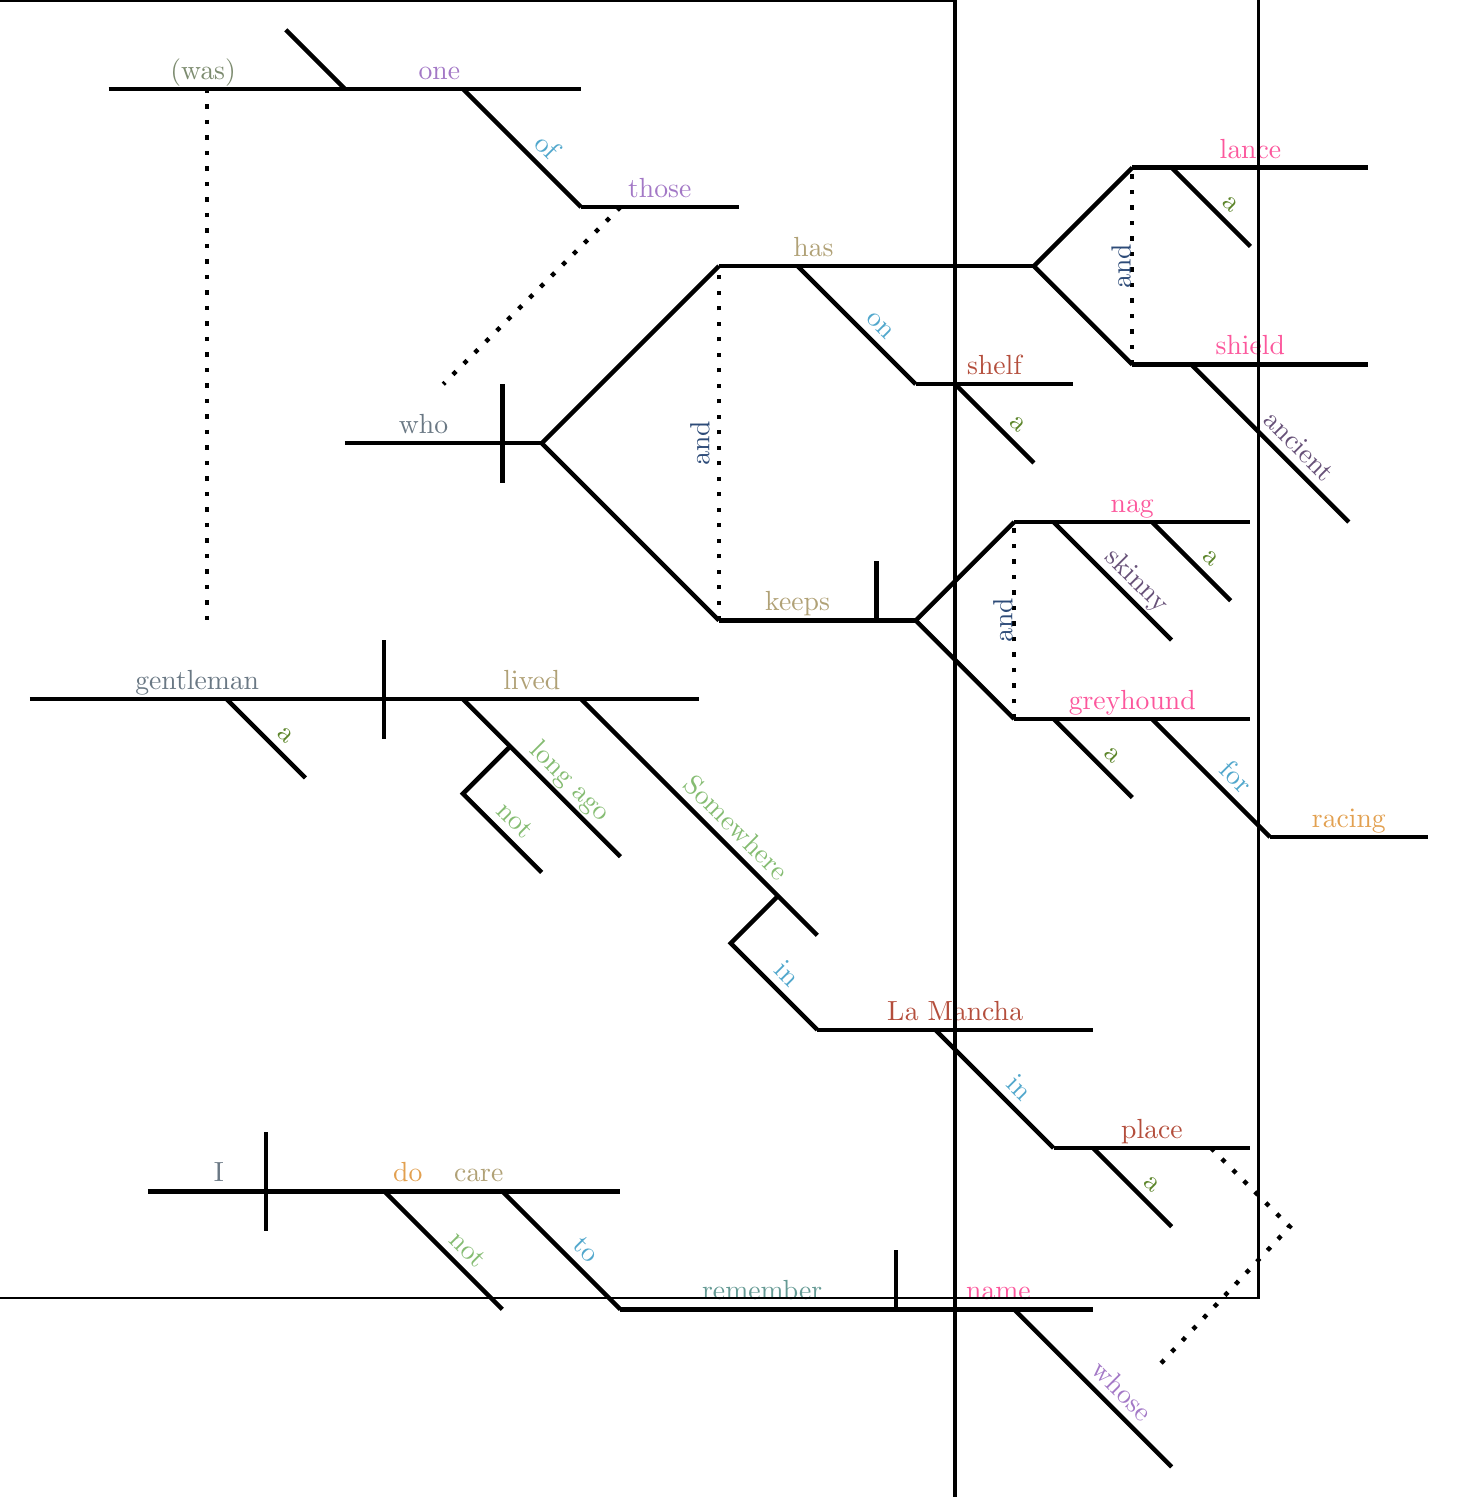
\begin{tikzpicture}
            \draw (-0.5, 16) -- (5.5, 16)
                node[pos=0.2, text=copula]{\strut (was)}
                node[pos=0.7, text=pronoun]{\strut one};
            \draw (1.75, 16.75) -- (2.5, 16);
            \draw (4, 16) -- (5.5, 14.5)
                node[sloped, pos=0.6, text=preposition]{\strut of};
            \draw (5.5, 14.5) -- (7.5, 14.5)
                node[pos=0.5, text=pronoun]{\strut those};
            \draw [loosely dotted] (6, 14.5) -- (3.75, 12.25);
            \draw [loosely dotted] (0.75, 16) -- (0.75, 9.25);

            \draw (2.5, 11.5) -- (5, 11.5)
                node[pos=0.4, text=subjectnoun]{\strut who};
            \draw (4.5, 12.25) -- (4.5, 11);

            \draw (5, 11.5) -- (7.25, 13.75);
            \draw (5, 11.5) -- (7.25, 9.25);
            \draw [loosely dotted] (7.25, 9.25) -- (7.25, 13.75)
                node[sloped, pos=0.5, text=conjunction]{\strut and};

            \draw (7.25, 13.75) -- (11.25, 13.75)
                node[pos=0.3, text=predicateverb]{\strut has};
            \draw (10.25, 14.5) -- (10.25, 13.75);
            \draw (8.25, 13.75) -- (9.75, 12.25)
                node[sloped, pos=0.6, text=preposition]{\strut on};
            \draw (9.75, 12.25) -- (11.75, 12.25)
                node[pos=0.5, text=noun]{\strut shelf};
            \draw (10.25, 12.25) -- (11.25, 11.25)
                node[sloped, pos=0.65, text=article]{\strut a};

            \draw (11.25, 13.75) -- (12.5, 15);
            \draw (11.25, 13.75) -- (12.5, 12.5);
            \draw [loosely dotted] (12.5, 12.5) -- (12.5, 15)
                node[above=-0.1cm, sloped, pos=0.5, text=conjunction]{\strut and};

            \draw (12.5, 15) -- (15.5, 15)
                node[pos=0.5, text=directobject]{\strut lance};
            \draw (13, 15) -- (14, 14)
                node[sloped, pos=0.6, text=article]{\strut a};
            \draw (12.5, 12.5) -- (15.5, 12.5)
                node[pos=0.5, text=directobject]{\strut shield};
            \draw (13.25, 12.5) -- (15.25, 10.5)
                node[sloped, pos=0.6, text=adjective]{\strut ancient};

            \draw (7.25, 9.25) -- (9.75, 9.25)
                node[pos=0.4, text=predicateverb]{\strut keeps};
            \draw (9.25, 10) -- (9.25, 9.25);

            \draw (9.75, 9.25) -- (11, 10.5);
            \draw (9.75, 9.25) -- (11, 8);
            \draw [loosely dotted] (11, 8) -- (11, 10.5)
                node[above=-0.1cm, sloped, pos=0.5, text=conjunction]{\strut and};

            \draw (11, 10.5) -- (14, 10.5)
                node[pos=0.5, text=directobject]{\strut nag};
            \draw (11.5, 10.5) -- (13, 9)
                node[sloped, pos=0.6, text=adjective]{\strut skinny};
            \draw (12.75, 10.5) -- (13.75, 9.5)
                node[sloped, pos=0.6, text=article]{\strut a};
            \draw (11, 8) -- (14, 8)
                node[pos=0.5, text=directobject]{\strut greyhound};
            \draw (11.5, 8) -- (12.5, 7)
                node[sloped, pos=0.6, text=article]{\strut a};
            \draw (12.75, 8) -- (14.25, 6.5)
                node[sloped, pos=0.6, text=preposition]{\strut for};
            \draw (14.25, 6.5) -- (16.25, 6.5)
                node[pos=0.5, text=verb]{\strut racing};

            \draw (-1.5, 8.25) -- (7, 8.25)
                node[pos=0.25, text=subjectnoun]{\strut gentleman}
                node[pos=0.75, text=predicateverb]{\strut lived};
            \draw (3, 9) -- (3, 7.75);
            \draw (1, 8.25) -- (2, 7.25)
                node[sloped, pos=0.6, text=article]{\strut a};
            \draw (4, 8.25) -- (6, 6.25)
                node[sloped, pos=0.6, text=adverb]{\strut long ago};
            \draw (4.6, 7.65) -- (4, 7.05) -- (5, 6.05)
                node[sloped, pos=0.5, text=adverb]{\strut not};
            \draw (5.5, 8.25) -- (8.5, 5.25)
                node[sloped, pos=0.6, text=adverb]{\strut Somewhere};
            
            \draw (8, 5.75) -- (7.4, 5.15) -- (8.5, 4.05)
                node[sloped, pos=0.5, text=preposition]{\strut in};
            \draw (8.5, 4.05) -- (12, 4.05)
                node[pos=0.5, text=noun]{\strut La Mancha};
            \draw (10, 4.05) -- (11.5, 2.55)
                node[sloped, pos=0.6, text=preposition]{\strut in};
            \draw (11.5, 2.55) -- (14, 2.55)
                node[pos=0.5, text=noun]{\strut place};
            \draw (12, 2.55) -- (13, 1.55)
                node[sloped, pos=0.6, text=article]{\strut a};
            \draw [loosely dotted] (13.5, 2.55) -- (14.5, 1.55) -- (12.85, -0.2);

            \draw (0, 2) -- (6, 2)
                node[pos=0.15, text=subjectnoun]{\strut I}
                node[pos=0.55, text=verb]{\strut do}
                node[pos=0.7, text=predicateverb]{\strut care};
            \draw (1.5, 2.75) -- (1.5, 1.5);
            \draw (3, 2) -- (4.5, 0.5)
                node[sloped, pos=0.6, text=adverb]{\strut not};
            \draw (4.5, 2) -- (6, 0.5)
                node[sloped, pos=0.6, text=preposition]{\strut to};
            \draw (6, 0.5) -- (12, 0.5)
                node[pos=0.3, text=infinitiveverb]{\strut remember}
                node[pos=0.8, text=directobject]{\strut name};
            \draw (9.5, 1.25) -- (9.5, 0.5);
            \draw (11, 0.5) -- (13, -1.5)
                node[sloped, pos=0.6, text=pronoun]{\strut whose};
        \end{tikzpicture}
    \end{sentencediagram}

    \begin{sentencediagram}{2}{1.75}{Stately, plump Buck Mulligan came from the stairhead, bearing\\a bowl of lather on which a mirror and a razor lay crossed.}{James Joyce}{Ulysses}
        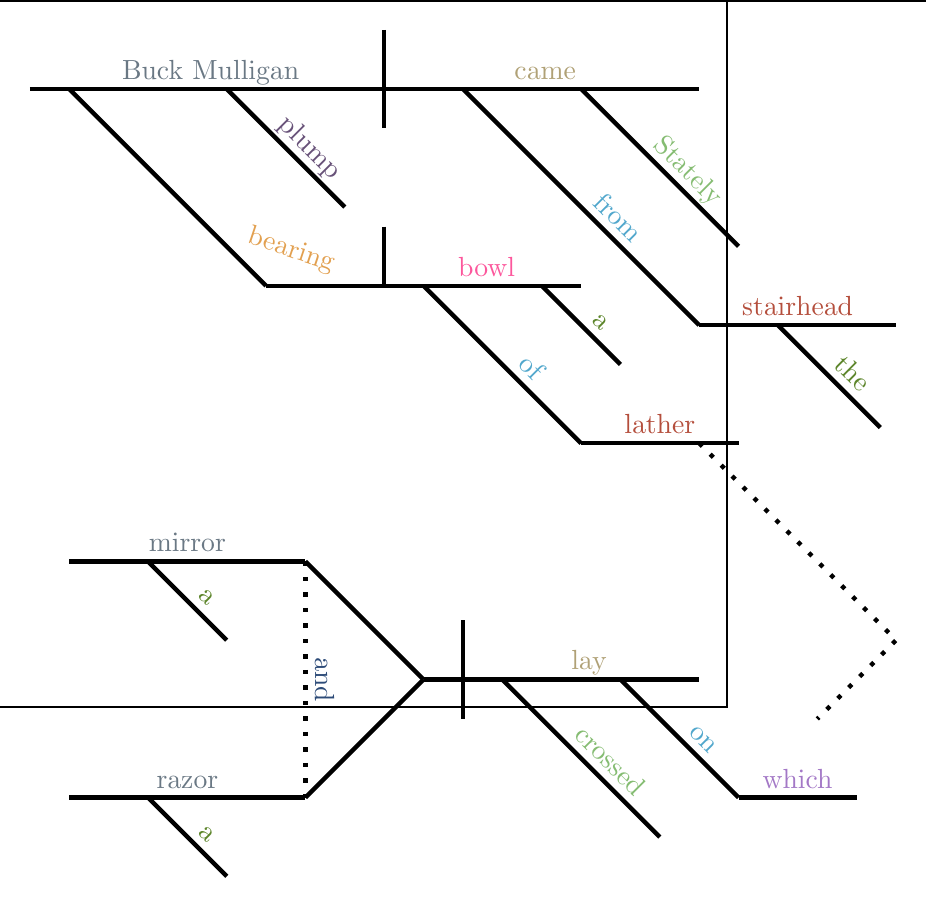
\begin{tikzpicture}
            \draw (-3.5, 6) -- (5, 6)
                node[pos=0.27, text=subjectnoun]{\strut Buck Mulligan}
                node[pos=0.77, text=predicateverb]{\strut came};
            \draw (-3, 6) -- (-0.5, 3.5);
            \draw (-1, 6) -- (0.5, 4.5)
                node[sloped, pos=0.6, text=adjective]{\strut plump};
            \draw (1, 6.75) -- (1, 5.5);
            \draw (2, 6) -- (5, 3)
                node[sloped, pos=0.6, text=preposition]{\strut from};
            \draw (5, 3) -- (7.5, 3)
                node[pos=0.5, text=noun]{\strut stairhead};
            \draw (6, 3) -- (7.3, 1.7)
                node[sloped, pos=0.6, text=article]{\strut the};
            \draw (3.5, 6) -- (5.5, 4)
                node[sloped, pos=0.6, text=adverb]{\strut Stately};

            \draw (-0.5, 3.5) -- (3.5, 3.5)
                node[pos=0.7, text=directobject]{\strut bowl};
            \path (-1, 4) -- (0.5, 3.5)
                node[sloped, pos=0.5, text=verb]{\strut bearing};
            \draw (1, 4.25) -- (1, 3.5);
            \draw (1.5, 3.5) -- (3.5, 1.5)
                node[sloped, pos=0.6, text=preposition]{\strut of};
            \draw (3.5, 1.5) -- (5.5, 1.5)
                node[pos=0.5, text=noun]{\strut lather};
            \draw (3, 3.5) -- (4, 2.5)
                node[sloped, pos=0.6, text=article]{\strut a};
            \draw[loosely dotted] (5, 1.5) -- (7.5, -1) -- (6.5, -2);

            \draw (-3, 0) -- (0, 0)
                node[pos=0.5, text=subjectnoun]{\strut mirror};
            \draw (-2, 0) -- (-1, -1)
                node[sloped, pos=0.6, text=article]{\strut a};
            \draw (-3, -3) -- (0, -3)
                node[pos=0.5, text=subjectnoun]{\strut razor};
            \draw (-2, -3) -- (-1, -4)
                node[sloped, pos=0.6, text=article]{\strut a};
            \draw (0, 0) -- (1.5, -1.5);
            \draw (0, -3) -- (1.5, -1.5);
            \draw[loosely dotted] (0, 0) -- (0, -3)
                node[sloped, pos=0.5, text=conjunction]{\strut and};

            \draw (1.5, -1.5) -- (5, -1.5)
                node[pos=0.6, text=predicateverb]{\strut lay};
            \draw (2, -0.75) -- (2, -2);
            \draw (2.5, -1.5) -- (4.5, -3.5)
                node[sloped, pos=0.6, text=adverb]{\strut crossed};
            \draw (4, -1.5) -- (5.5, -3)
                node[sloped, pos=0.6, text=preposition]{\strut on};
            \draw (5.5, -3) -- (7, -3)
                node[pos=0.5, text=pronoun]{\strut which};
        \end{tikzpicture}
    \end{sentencediagram}
\end{document}
